
\subsection{Felix (Flexible blokken)}\label{felix}
Het is voor eindredacteuren mogelijk om blokken de plaatsen op pagina's. Hiermee krijgt de redacteur enige vrijheid over de indeling van de pagina. Hier zijn wel beperkingen van toepassing volgens het grafisch ontwerp.

Door met de muis over de grijze balk te gaan verschijnt er een tandwieltje, als je daarop klikt dan verschijnt er een optie \emph{Blok toevoegen}. Hier kan een keuze gemaakt worden om een enkel item weer te geven op de website, dit zijn \emph{Nodetypes}, of een aantal items, zoals bijvoorbeeld \emph{Het laatste nieuws}.

\begin{center}
	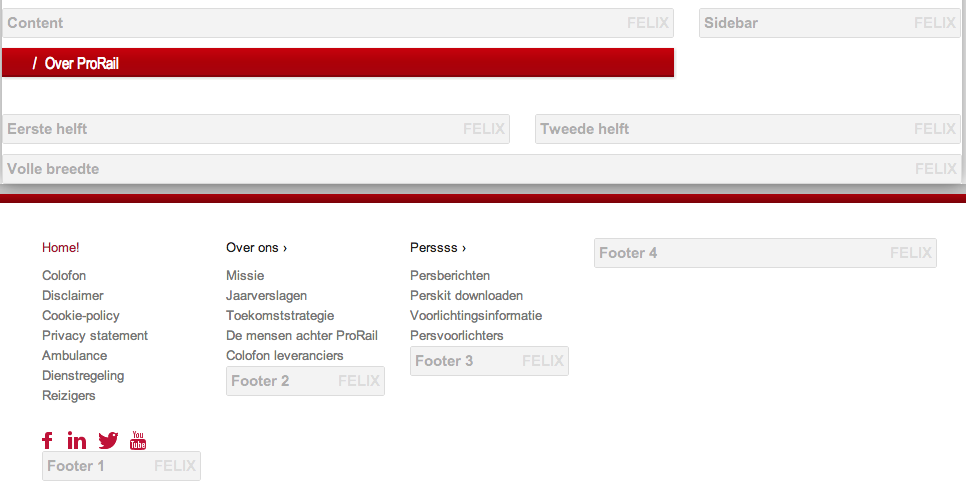
\includegraphics[width=\textwidth]{img/felix.png}
\end{center}

\subsubsection{Felix blok titel aanpassen}\label{felixbloktitel}

De titel van een felix blok kan altijd aangepast worden. Om dit te doen klik je op het \emph{tandwieltje} en vervolgens op \emph{Eigenschappen aanpassen}. Vul bij het veld \emph{Onderwerp} de gewenste titel in, laat het veld leeg om de standaard waarde te gebruiken. Klik op de knop \emph{Opslaan} om de titel op te slaan. 

\begin{center}
	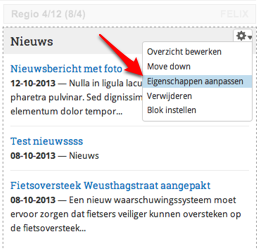
\includegraphics[scale=1.0]{img/felix0.png}
\end{center}

\subsubsection{Felix blok volgorde aanpassen}\label{felixblokvolgorde}

Klik op het \emph{tandwieltje} en klik vervolgens op \emph{Verplaats omhoog} of op \emph{Verplaats omlaag} om het blok 1 positie omhoog of omlaag te verplaatsen. De nieuwe blok volgorde zal automatisch opgeslagen worden.

\begin{center}
	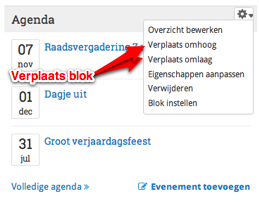
\includegraphics[scale=1.0]{img/felix3.png}
\end{center}

\subsubsection{Felix regio's}\label{felixregios}

De onderstaande afbeeldingen tonen alle felix regio's. Dit zijn gebieden op de website waar blokken aan toegevoegd kunnen worden. Op de afbeeldingen zie je aanduidingen als \emph{Regio 8/12} en \emph{Regio 4/12}, dit slaat op de breedte van de regio. De gehele pagina bestaat uit 12 kolommen, \emph{Regio 8/12} neemt dus 8 van de 12 kolommen in. Het is niet aangeraden om hele brede blokken (bijv. Carrousel breed 9/12) toe te voegen aan hele smalle regio's (bijv. Regio 4/12). Als je dit toch doet kan het zijn dat de opmaak van de website niet meer klopt.

\begin{center}
	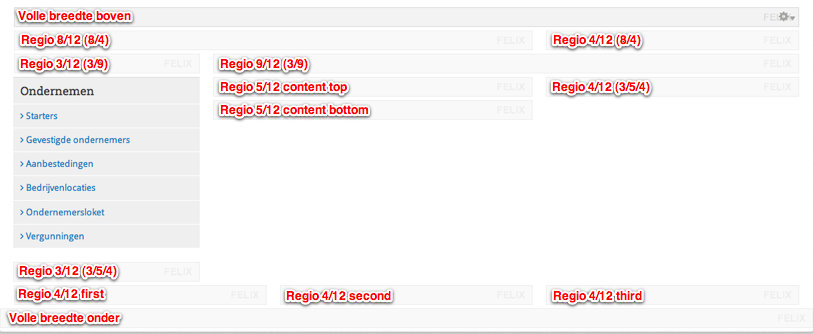
\includegraphics[width=\textwidth]{img/felix1.png}
\end{center}

\begin{center}
	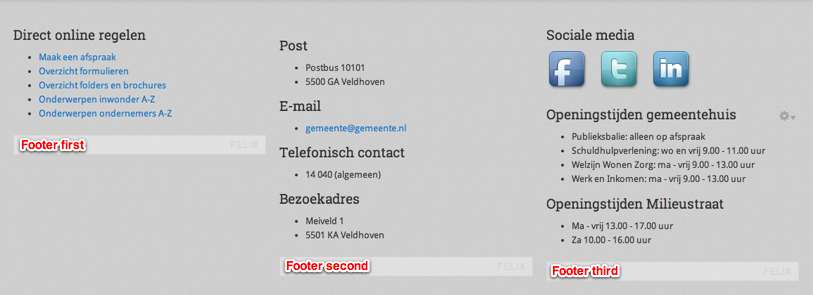
\includegraphics[width=\textwidth]{img/felix2.png}
\end{center}

\subsubsection{Felix blokken}\label{felixblokken}

Felix blokken zijn de daadwerkelijke flexibele blokken, deze specifieke blokken kunnen overal op de website en in alle felix regio's getoond worden.

\textbf{Nodetype}

\begin{itemize}
\item Editorial
\item Peiling
\item Slide 
\item Webformulier
\end{itemize}

\textbf{Block}

\begin{itemize}
\item Subnavigatie voorbeeld
\end{itemize}

\textbf{Menu}

\begin{itemize}
\item Toptaken
\end{itemize}

\textbf{Menu Block}

\begin{itemize}
\item Subnavigatie
\end{itemize}

\textbf{Quicktabs}

\begin{itemize}
\item Nieuws Agenda tabblok
\end{itemize}

\textbf{Submenu Tree}

\begin{itemize}
\item Sibling content
\item Extended menu links
\end{itemize}

\textbf{Views}

\begin{itemize}
\item Agenda teaserblok
\item Agenda lijstblok
\item Berichtenblok
\item Teamdocumentenblok
\item Favorietenblok
\item Fotoalbumblok
\item Google maps kaart
\item Marktplaats lijstblok
\item Marktplaats gevraagd blok
\item Marktplaats aangeboden blok
\item Marktplaats gevraagd pagina
\item Marktplaats aangeboden pagina
\item Nieuws teaserblok
\item Nieuws lijstblok
\item Nieuws lijstblok + afbeelding
\item Carrousel breed (9/12)
\item Carrousel smal (4/12)
\item Personenblok intranet
\item Personenblok internet
\item Teamledenblok
\item Productenblok
\item Regelingenblok
\item Updatesblok
\item Recent FAQs
\item Overige onderwerpenblok
\item Weblog blok
\end{itemize}